\def\CTeXPreproc{Created by ctex v0.2.9, don't edit!}
%\documentclass{beamer}
\documentclass[%handout,
xcolor=pdftex]{beamer}
\mode<presentation> {
  \usetheme{Warsaw}
  \setbeamercovered{transparent}
}
\let\Tiny=\tiny
\usetheme{Singapore}
\usecolortheme{dolphin}
\usepackage{amsmath}
\usepackage{textcomp}
\usepackage{amssymb}
\usepackage{amsthm}
\usepackage{graphicx}
\usepackage{color}
\usepackage{lipsum}
\usepackage{hyperref}
\usepackage{multirow}
\usepackage{bm}
\DeclareMathSymbol{\Phi}{\mathalpha}{operators}{8}
%\setbeamertemplate{headline}{}
\setbeamertemplate{footline}[page number]
\newcommand\Fontvi{\fontsize{9pt}{8}\selectfont}
\newcommand\Fontvii{\fontsize{7pt}{8}\selectfont}
\newcommand{\backupbegin}{
   \newcounter{finalframe}
   \setcounter{finalframe}{\value{framenumber}}
}
\newcommand{\backupend}{
   \setcounter{framenumber}{\value{finalframe}}
}\newtheorem{proposition}{Proposition}
\title{Unit 18: Spectral Density}
\author[STAT 5170: Applied Time Series, Unit 18]{Jeffrey Woo}
\institute{Department of Statistics, University of Virginia}
\date{Spring 2020} %ADD LECTURE 21 FROM ADITYA

\AtBeginSubsection[] {
  \begin{frame}<beamer>{Outline}
    \tableofcontents[currentsection,currentsubsection]
  \end{frame}
}



\begin{document}


\frame{\titlepage}


\begin{frame}
\frametitle{Readings for Unit 18}

Textbook chapter 4.2 (until page 175).

\end{frame}



\begin{frame}
\frametitle{Last Unit}
\begin{enumerate}
\item Introduction to Spectral Analysis.
\end{enumerate}
\end{frame}

\begin{frame}
\frametitle{This Unit}
\begin{enumerate}
\item Spectral Density: Fourier Transformation of Autocovariance.
\item Properties of Spectral Density.
\end{enumerate}
\end{frame}

\begin{frame}
\frametitle{Motivation}

The spectral density is a Fourier transform of the autocovariance function $\gamma(h)$. Autocovariance is in terms of \underline{\hspace{8mm}} whereas spectral density is in terms of \underline{\hspace{10 mm}}.

\end{frame}

\section{Spectral Density}
\frame{\tableofcontents[currentsection]}

\begin{frame}
\frametitle{Transformation}

Consider a transformation from Celsius to Fahrenheit: $F = 1.8C + 32$. \\
\vspace{5mm}
To transform back, we use $C = \frac{F-32}{1.8}$. We don't really lose any information during the transformation.

\end{frame}

\begin{frame}
\frametitle{Fourier Transform}


We move between a function on the integers $...,-2,-1,0,1,2,...$ and a function in the frequency space. So, for
a function $a_t, t=...,-2,-1,0,1,2,...$ we can move to the
frequency space by taking the Fourier transform
\begin{eqnarray*}
A(\omega) = \sum_{t=-\infty}^{\infty} a_t e^{-2 \pi i \omega t}, -0.5\leq \omega \leq 0.5.
\end{eqnarray*}

We can then go backwards using $a_t=\int_{-0.5}^{0.5} A(\omega) e^{2
\pi i \omega t} d\omega$ for each $t$.

\end{frame}

\begin{frame}
\frametitle{Spectral Density}

If the autocovariance function, $\gamma(h)$, of a stationary process satisfies $\sum_{h=-\infty}^{\infty}  |\gamma(h)| < \infty$, then it has the representation

\begin{equation} \label{eq:inverse}
\gamma(h) = \int^{1/2}_{-1/2} f(\omega) e^{2\pi i\omega h} d\omega, \quad h=0,\pm 1,\pm 2,\ldots.
\end{equation}

(\ref{eq:inverse}) is called the \underline{\hspace{70 mm}}. The \underline{\hspace{25 mm}} is denoted by

\begin{equation} \label{eq:spec}
f(\omega)  = \sum^\infty_{h=-\infty} \gamma(h) e^{-2\pi i\omega h}, \quad -1/2 \leq \omega \leq 1/2.
\end{equation}

Autocovariance is in terms of \underline{\hspace{8 mm}} whereas spectral density is in terms of \underline{\hspace{10 mm}}.


\end{frame}


\begin{frame}
\frametitle{Spectral Density}

\begin{itemize}
\item The spectral density, (\ref{eq:spec}), provides information about the relative strengths of the various frequencies for \underline{\hspace{18 mm}} \underline{\hspace{25 mm}} in the time series.
\item The spectral density is also called the power spectrum.  
\item Remember
that $\gamma(h)$ completely determines the distribution for a
stationary Gaussian process.  So, the spectral density also
completely determines the distribution for a
stationary Gaussian process.
\end{itemize}

\end{frame}

\begin{frame}
\frametitle{Spectral Density}


Notice that when $h=0$, from (\ref{eq:inverse}), we have

\begin{equation} \label{eq:var}
\gamma(0) = \mbox{Var}(x_t) = \int^{1/2}_{-1/2} f(\omega) d\omega.
\end{equation}

An interpretation of (\ref{eq:var}) is that the ``total" integrated spectral density equals the variance of the time series.  Thus the spectral density within a particular interval of frequencies can be viewed as the amount of the variance \underline{\hspace{15 mm}} by those frequencies.

\end{frame}


\begin{frame}
\frametitle{Trigonometric Properties}

Recall that

\begin{itemize}
\item a cosine function is \underline{\hspace{8 mm}}, i.e. $\cos(-\theta) = \cos(\theta)$.
\item a sine function is \underline{\hspace{7 mm}}, i.e. $\sin(-\theta) = -\sin(\theta)$.
\end{itemize}

\end{frame}

\begin{frame}
\frametitle{Euler's Formula}

Recall Euler's formula:

\begin{equation} \label{eq:euler}
e^{i \alpha} = \cos (\alpha) + i \sin (\alpha).
\end{equation}

Consequently,

\begin{equation} \label{eq:ecos}
\cos(\alpha) = \frac{e^{-i \alpha} + e^{i \alpha}}{2}
\end{equation}

and

\begin{equation} \label{eq:esin}
\sin(\alpha) = \frac{e^{i \alpha} - e^{-i \alpha}}{2i}.
\end{equation}


\end{frame}

\begin{frame}
\frametitle{Derivation of Inverse Transformation of Spectral Density}



\end{frame}



\section{Properties of Spectral Density}
\frame{\tableofcontents[currentsection]}

\begin{frame}
\frametitle{Properties of Spectral Density}

\begin{enumerate}
%\item $f(\omega)$ is periodic, with period 1.
\item $f(\omega) \geq 0$ because $\gamma(h)$ is non-negative definite.
\item $f(\omega)$ is even, i.e. $f(\omega) = f(-\omega)$.
\item $f(\omega) = f(\omega+1)$.
\end{enumerate}



\end{frame}

\begin{frame}
\frametitle{Derivation of Properties}



\end{frame}

\begin{frame}
\frametitle{Derivation of Properties}



\end{frame}



\section{Worked Examples}
\frame{\tableofcontents[currentsection]}



\begin{frame}
\frametitle{Spectral Density of White Noise}



\end{frame}

\begin{frame}
\frametitle{Spectral Density of White Noise}

This means all frequencies receive equal weight. This is analogous to the spectrum of white light, where all colors enter equally in white light. (Hence the term white noise!)


\end{frame}

\begin{frame}
\frametitle{Spectral Density of MA(1)}



\end{frame}

\begin{frame}
\frametitle{Spectral Density of MA(1)}

\textbf{Question}: Suppose $\theta=0.5$ and $\sigma_w^2=1$, sketch the power spectrum.

\vspace{40mm}

What is the implication of this power spectrum?

\end{frame}

\begin{frame}
\frametitle{Time Series Plot of MA(1)}


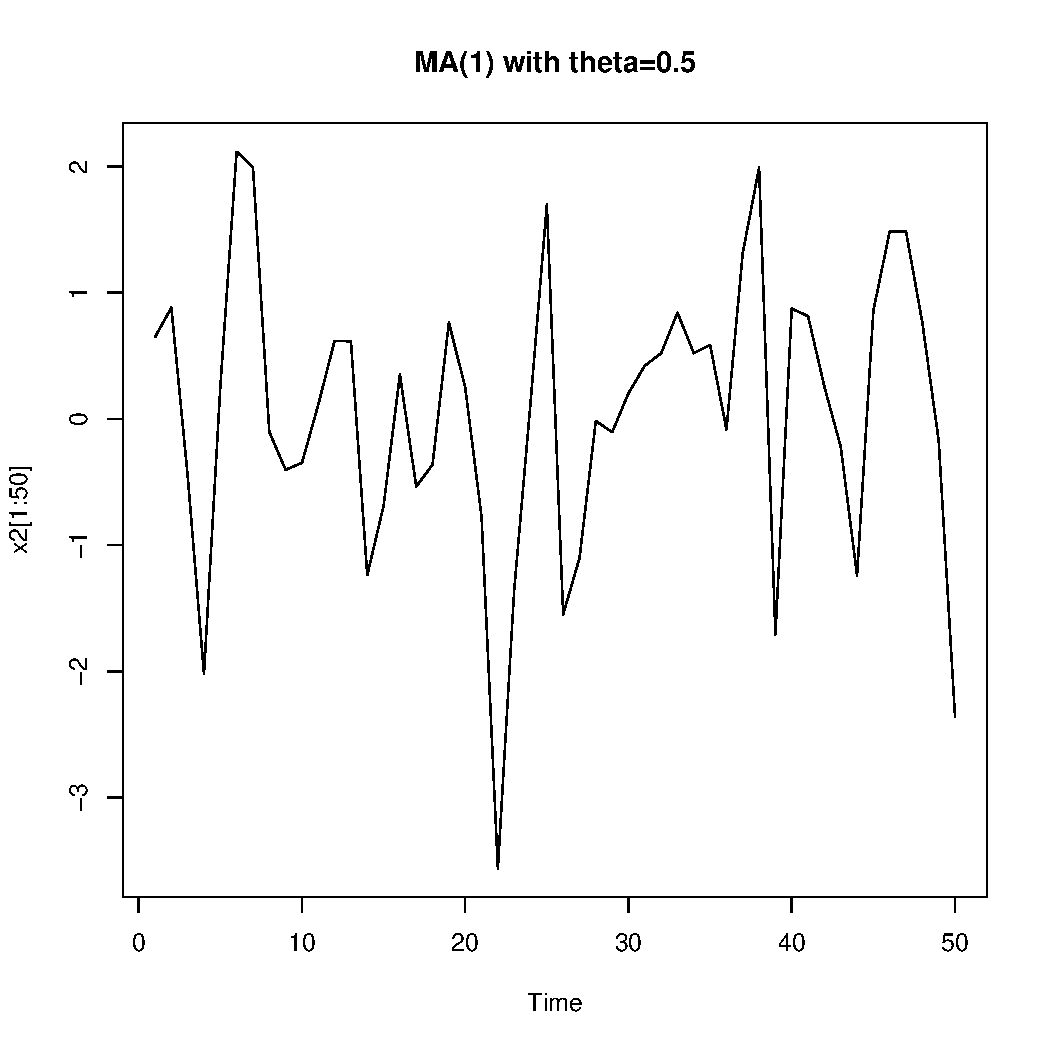
\includegraphics[width=100mm, height=80mm]{ma1_1ts.pdf}


\end{frame}

\begin{frame}
\frametitle{Spectral Density of MA(1)}

Power spectrum of MA(1) when $\theta=-0.5$ and $\sigma_w^2=1$.

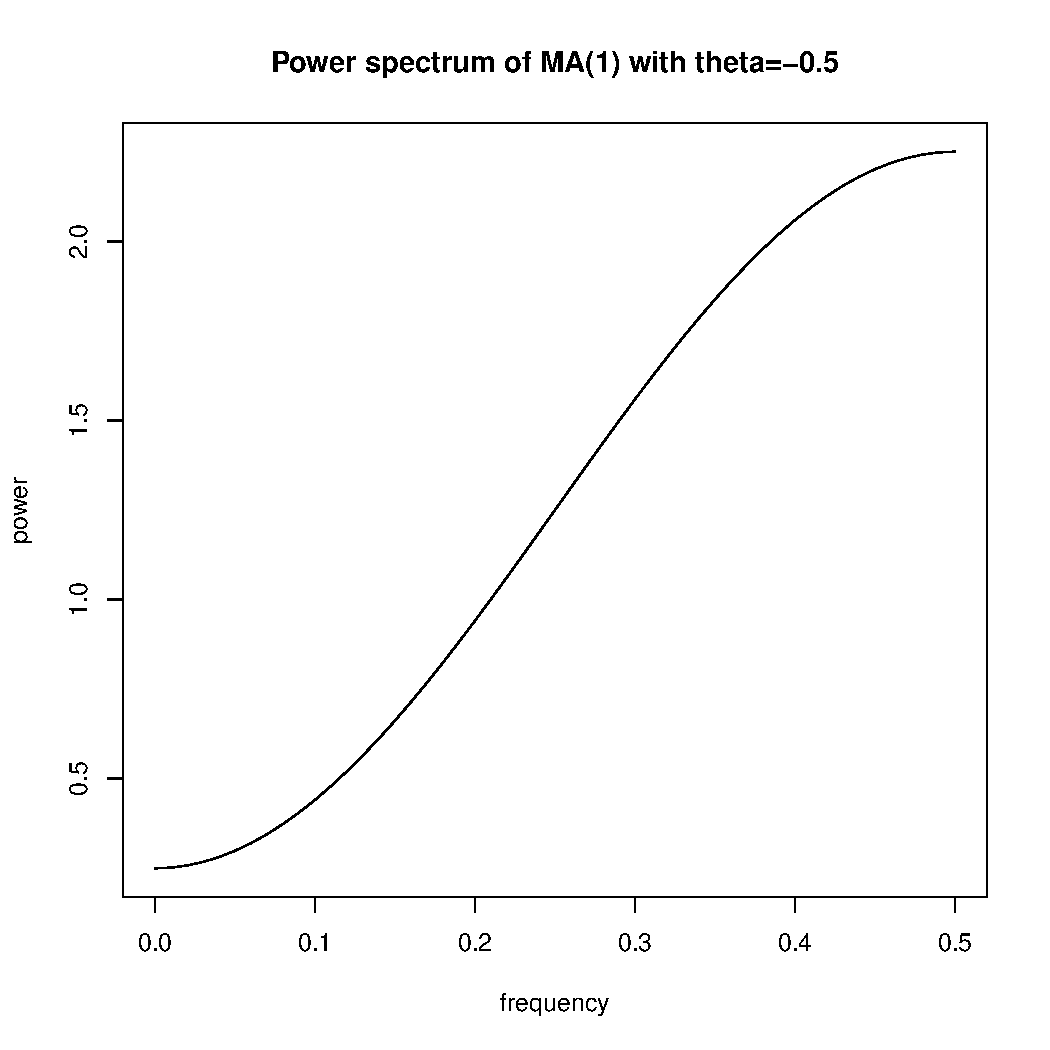
\includegraphics[width=100mm, height=80mm]{ma1_2power.pdf}

\end{frame}

\begin{frame}
\frametitle{Time Series Plot of MA(1)}


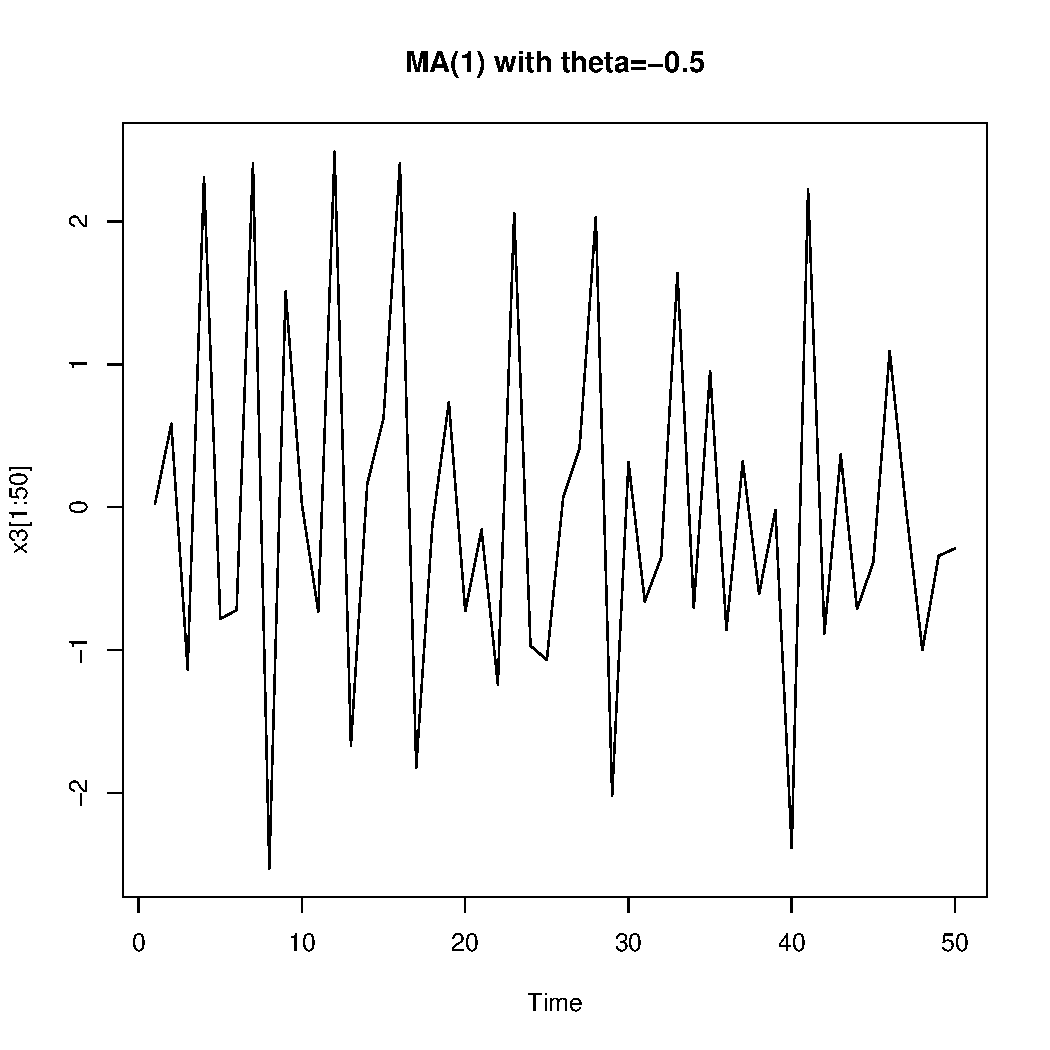
\includegraphics[width=100mm, height=80mm]{ma1_2ts.pdf}


\end{frame}

\begin{frame}
\frametitle{ACF of MA(1)}

\textbf{Question}: How are the ACF plots of an MA(1) process different when $\theta=0.5$ versus $\theta=-0.5$? Does this difference provide an explanation to the difference in their time series plots?

\end{frame}

\begin{frame}
\frametitle{Spectral Density of AR(1)}



\end{frame}




\end{document} 